% ============================================================
%  Figure : Pipeline de préparation des données (DatasetBuilder)
%  Compiler : pdflatex fig_pipeline.tex
% ============================================================
\documentclass[tikz, border=8pt]{standalone}

\usepackage[utf8]{inputenc}
\usepackage[T1]{fontenc}
\usepackage{xcolor}
\usepackage{tikz}
\usetikzlibrary{positioning, arrows.meta, fit, backgrounds}

\definecolor{pythonblue}{HTML}{356D9C}
\definecolor{pythonyellow}{HTML}{FED03E}
\definecolor{pythondark}{HTML}{1E4068}
\definecolor{pythonlight}{HTML}{D6E8F5}

\begin{document}
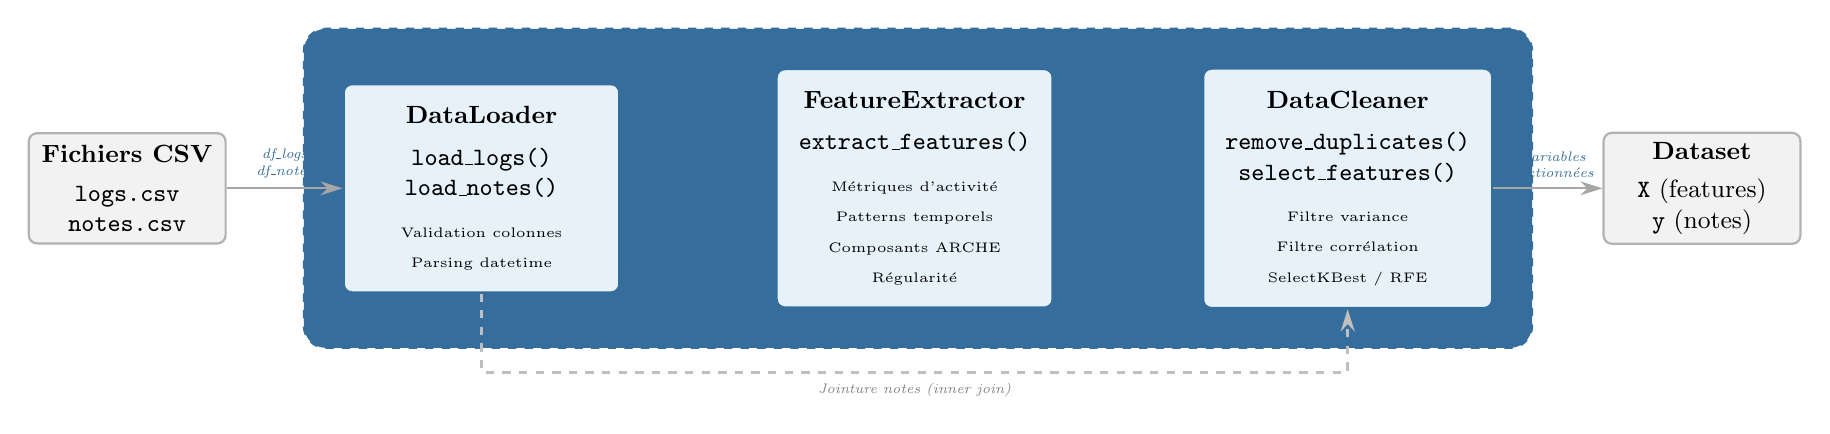
\begin{tikzpicture}[
  component/.style={
    draw=pythonblue, fill=white, thick,
    minimum width=3.5cm, minimum height=2.2cm,
    align=center, font=\small, rounded corners=3pt,
    inner sep=8pt
  },
  io/.style={
    draw=gray!60, fill=gray!10, thick,
    minimum width=2.5cm, minimum height=1.4cm,
    align=center, font=\small, rounded corners=3pt
  },
  arrow/.style={-{Stealth[length=8pt, width=5pt]}, very thick, pythonblue},
  ioarrow/.style={-{Stealth[length=8pt, width=5pt]}, thick, gray!70},
  label/.style={font=\tiny\itshape, color=pythonblue, align=center}
]

% ---- Entrée ----
\node[io] (csv) at (-4.5, 0) {
  \textbf{Fichiers CSV}\\[3pt]
  \texttt{logs.csv}\\
  \texttt{notes.csv}
};

% ---- DataLoader ----
\node[component, fill=pythonlight!60] (dl) at (0, 0) {
  \textbf{DataLoader}\\[4pt]
  \texttt{load\_logs()}\\
  \texttt{load\_notes()}\\[4pt]
  \tiny Validation colonnes\\
  \tiny Parsing datetime
};

% ---- FeatureExtractor ----
\node[component, fill=pythonlight!60] (fe) at (5.5, 0) {
  \textbf{FeatureExtractor}\\[4pt]
  \texttt{extract\_features()}\\[4pt]
  \tiny Métriques d'activité\\
  \tiny Patterns temporels\\
  \tiny Composants ARCHE\\
  \tiny Régularité
};

% ---- DataCleaner ----
\node[component, fill=pythonlight!60] (dc) at (11, 0) {
  \textbf{DataCleaner}\\[4pt]
  \texttt{remove\_duplicates()}\\
  \texttt{select\_features()}\\[4pt]
  \tiny Filtre variance\\
  \tiny Filtre corrélation\\
  \tiny SelectKBest / RFE
};

% ---- Sortie ----
\node[io] (out) at (15.5, 0) {
  \textbf{Dataset}\\[3pt]
  \texttt{X} (features)\\
  \texttt{y} (notes)
};

% Flèches entre composants
\draw[ioarrow] (csv.east) -- (dl.west)
  node[midway, above, label]{df\_logs\\df\_notes};

\draw[arrow] (dl.east) -- (fe.west)
  node[midway, above, label]{df\_logs};

\draw[arrow] (fe.east) -- (dc.west)
  node[midway, above, label]{df\_features\\(1 ligne/étudiant)};

\draw[ioarrow] (dc.east) -- (out.west)
  node[midway, above, label]{k variables\\sélectionnées};

% Jointure notes (flèche depuis DataLoader vers DataCleaner via le bas)
\draw[arrow, gray!50, dashed] (dl.south) -- ++(0, -1.0)
  -- node[below, label, color=gray]{Jointure notes (inner join)} ++(11, 0)
  -- (dc.south);

% ---- Boîte DatasetBuilder (façade) ----
\begin{scope}[on background layer]
  \node[
    draw=pythondark, dashed, thick,
    fill=pythonyellow!8,
    rounded corners=8pt,
    fit=(dl)(fe)(dc),
    inner sep=14pt,
    label={[font=\bfseries\small\color=pythondark]above:DatasetBuilder \textit{(Façade)}}
  ] (dsb) {};
\end{scope}

\end{tikzpicture}
\end{document}
